\documentclass[11pt,a4paper]{article}
\usepackage[T1]{fontenc}
\usepackage{mathpazo}
\usepackage[scaled=0.9]{helvet}
\usepackage{amsmath}
\usepackage[a4paper,margin=24mm,top=22mm,bottom=26mm]{geometry}
\usepackage{microtype}
\usepackage{graphicx}
\usepackage{booktabs}
\usepackage{tabularx}
\usepackage{xcolor}
\usepackage{enumitem}
\usepackage{tikz}
\usetikzlibrary{arrows.meta,positioning}
\usepackage[font=small,labelfont=bf,labelsep=period]{caption}
\usepackage{titlesec}
\usepackage{fancyhdr}
\usepackage[hidelinks]{hyperref}

\definecolor{ink}{HTML}{1B2733}
\definecolor{gbt}{HTML}{2A78D6}
\definecolor{net}{HTML}{EB6834}
\definecolor{chk}{HTML}{1BAF7A}
\definecolor{muted}{HTML}{5B6675}

\titleformat{\section}{\normalfont\Large\bfseries\color{ink}}{\thesection}{0.8em}{}
\titleformat{\subsection}{\normalfont\large\bfseries\color{ink}}{\thesubsection}{0.8em}{}
\titlespacing*{\section}{0pt}{16pt}{6pt}
\titlespacing*{\subsection}{0pt}{11pt}{4pt}
\setlength{\parskip}{3pt}
\widowpenalty=10000 \clubpenalty=10000
\setlist{itemsep=1pt,topsep=3pt}
\renewcommand{\arraystretch}{1.15}

\pagestyle{fancy}\fancyhf{}
\renewcommand{\headrulewidth}{0pt}
\fancyfoot[L]{\footnotesize\color{muted}A.\,M.~Elsayed \,--\, Paper 2 progress report}
\fancyfoot[R]{\footnotesize\color{muted}\thepage}

\newcommand{\pc}{\,\%}
\newcommand{\Ncr}{N_{\mathrm{cr}}}

\begin{document}

\begin{center}
{\small\color{muted}Progress report on Paper 2 \quad|\quad 25 November 2026}\\[10pt]
{\LARGE\bfseries\color{ink} Physics-informed neural networks with a certified\\[2pt] GBT check for the buckling of stiffened composite panels\par}
\vspace{10pt}
{\large Aya Medhat Elsayed}\\[2pt]{\small\color{muted}Institute for Lightweight Engineering and Structural Mechanics (LSM), TU Darmstadt}
\end{center}

\vspace{4pt}
\begin{abstract}
\noindent This report follows the machine-learning work on the second paper of my project, from the first physics-informed network on 22 October to the cost study of 23 November 2026, including every attempt that did not work. The physics is our periodic Generalized Beam Theory (GBT) code, which replaces the plate model and the Abaqus oracle of Paper~1. I built a shared reduced space in which every design has the same coordinates, found that a physics-only network trains only after its numerical conditioning is fixed, compared physics, data and hybrid losses, tried one network for all lay-ups and split it into lay-up experts, and finally compared the network honestly with simple alternatives. The network's modes start a block eigen-iteration whose relative residual gives a label-free error estimate. With 120 labels, the instant answer of the network is within 0.24--1.18\pc{} of full GBT on 320 unseen designs; the error estimate was never below the true error in 3800 checks, and a 5\pc{} target is met on every design without labels. The network adds less than I expected; the main contribution is the certified GBT check.
\end{abstract}

\section{Starting point and aim}

In Paper~1 \cite{p1} I predicted the local buckling of omega-stringer panels with a hybrid physics-informed neural network (PINN). Two small one-dimensional networks described the skin and the foot strips with one sine wave along the panel, the plate energy used the reduced bending stiffness (RBS) approximation, and each panel was trained on its own. Suspicious answers, flagged when the load left a window of $-15\pc{}/{+3}\pc{}$ around the previous panel, were checked with Abaqus, and an MLP on the stringer pitch $b_s$ and the aspect ratio $\beta$ gave fast answers for one cross-ply lay-up.

The paper worked, but it left four weak points: at the tight pitch $b_s = 124.25$\,mm the error against Abaqus grew to 10.30\pc{} on average and 14.54\pc{} at most in its $\beta$ sweep (Paper~1, Table~1) and to 10.80\pc{} in its independent Abaqus test (Table~2), because of the RBS approximation; Abaqus as oracle is expensive and lies outside the framework; the window depends on the order in which panels are asked; and the tool covered one lay-up only. For Paper~2 I set five goals: (1)~GBT as the physics, (2)~the GBT code instead of Abaqus, (3)~a reasonable check instead of the window, (4)~the lay-up as part of the tool, and (5)~a fast tool. Two rules were fixed from the start: the network must remain a PINN, with labels only as support, and every answer may depend only on the design itself.

\begin{figure}[t]
\centering
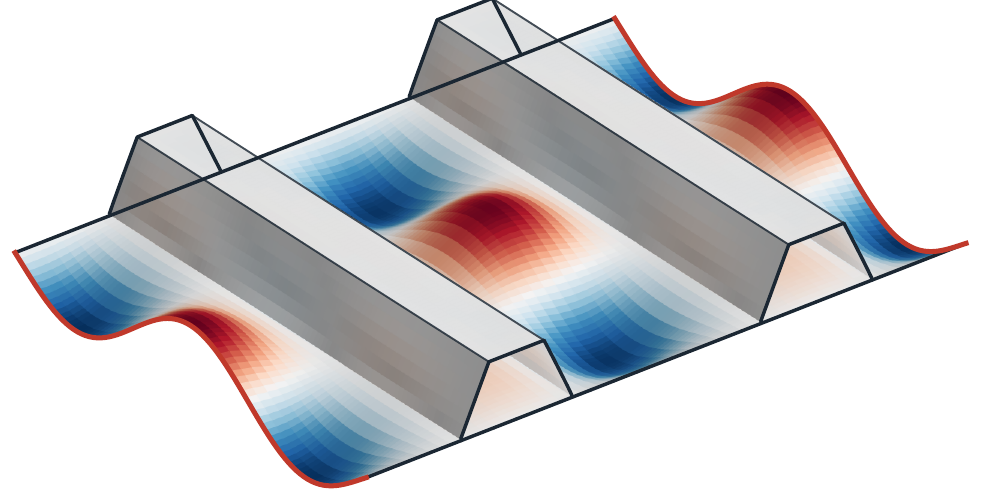
\includegraphics[width=0.78\textwidth]{panel_mode.png}
\caption{Periodic omega-stringer cell and its critical buckling mode from GBT (``Unsym'' cell of the GBT paper \cite{gbt}, $b_s=150$\,mm, $\beta=1.5$, simply supported ends, $\Ncr=32.26$\,N/mm). Modes of this kind are what the network has to predict.}
\label{fig:panel}
\end{figure}

\section{The tool in brief}

Figure~\ref{fig:tool} shows the tool as it stands now. The physics is the shear-deformable periodic GBT formulation of our GBT paper \cite{gbt,sc}, which agrees with Abaqus within 0.57--0.64\pc{} on average for periodic cells. Every design is described in one shared reduced space, a POD basis of 241 cross-section modes times a dictionary of longitudinal functions, so that the stiffness matrix $\mathbf K$ and the geometric matrix $\mathbf G$ of any design have the same size and meaning. A small network for each lay-up and side condition maps $(b_s,\beta)$ to eight candidate modes and an instant value of $\Ncr$. The modes then start a block LOBPCG iteration \cite{lobpcg} in the reduced space of the design; each iterate is an upper bound of the critical load of the reduced model (which is at most 0.49\pc{} from full GBT over 1064 designs), and the iteration stops when the relative residual $\eta=\lVert\mathbf G\mathbf x-\mu\mathbf K\mathbf x\rVert_{\mathbf M^{-1}}/\mu$ falls below a chosen tolerance. Table~\ref{tab:setup} gives the set-up of the final study.

\begin{figure}[t]
\centering
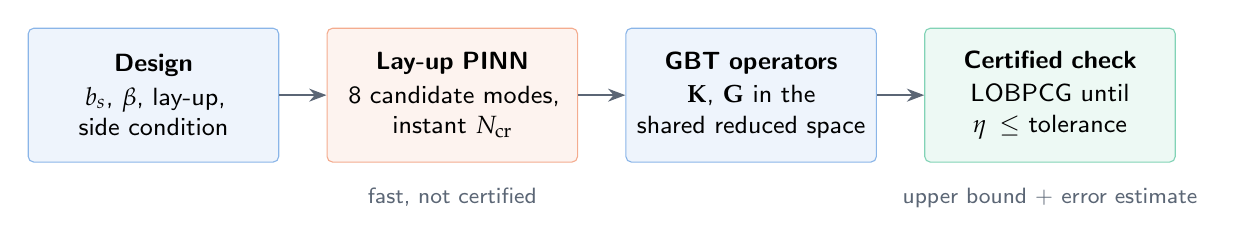
\begin{tikzpicture}[font=\sffamily\small, node distance=6mm,
  bx/.style={draw=#1!55, fill=#1!8, rounded corners=2pt, align=center, text width=29mm, minimum height=17mm, inner sep=4pt},
  ar/.style={-{Stealth[length=2.2mm]}, draw=muted, line width=0.6pt}]
\node[bx=gbt] (d) {\textbf{Design}\\[1pt] $b_s$, $\beta$, lay-up,\\ side condition};
\node[bx=net, right=of d] (n) {\textbf{Lay-up PINN}\\[1pt] 8 candidate modes,\\ instant $\Ncr$};
\node[bx=gbt, right=of n] (o) {\textbf{GBT operators}\\[1pt] $\mathbf K$, $\mathbf G$ in the\\ shared reduced space};
\node[bx=chk, right=of o] (c) {\textbf{Certified check}\\[1pt] LOBPCG until\\ $\eta\le$ tolerance};
\draw[ar] (d)--(n); \draw[ar] (n)--(o); \draw[ar] (o)--(c);
\node[below=2mm of n, font=\sffamily\footnotesize, text=muted] {fast, not certified};
\node[below=2mm of c, font=\sffamily\footnotesize, text=muted] {upper bound $+$ error estimate};
\end{tikzpicture}
\caption{The tool: the network gives an instant answer and starting modes; the GBT check turns them into a certified load.}
\label{fig:tool}
\end{figure}

\begin{table}[t]
\centering\small
\caption{Set-up of the final study.}
\label{tab:setup}
\begin{tabularx}{\textwidth}{@{}lX@{}}
\toprule
Panel & omega-stringer panel, periodic cell, simply supported loaded ends \\
Design inputs & $b_s = 124.25$--$285.5$\,mm, $\beta = a/b_s = 0.75$--$3.5$ \\
Lay-ups (skin) & cross-ply $[0/90/0/90]_s$, quasi-isotropic $[45/{-45}/0/90]_s$, $0^\circ$-rich $[45/0/{-45}/0]_s$, $\pm45^\circ$ $[45/{-45}/{-45}/45]_s$ \\
Side conditions & symmetry line (half pitch) and periodic cell (two pitches) \\
Data per expert & 152 training and validation designs (up to 120 with labels), 40 unseen test designs \\
Reference & full GBT solution of every test design \\
\bottomrule
\end{tabularx}
\end{table}

\section{The machine-learning journey}

Figure~\ref{fig:history}a shows the phases of the work and Figure~\ref{fig:history}b how the error of the network developed from test to test. The instant answer moved between 140\pc{} and 0.24\pc, while the answer after a few physics steps stayed below 0.5\pc{} on average in every test. The subsections follow the order in which things happened.

\begin{figure}[t]
\centering
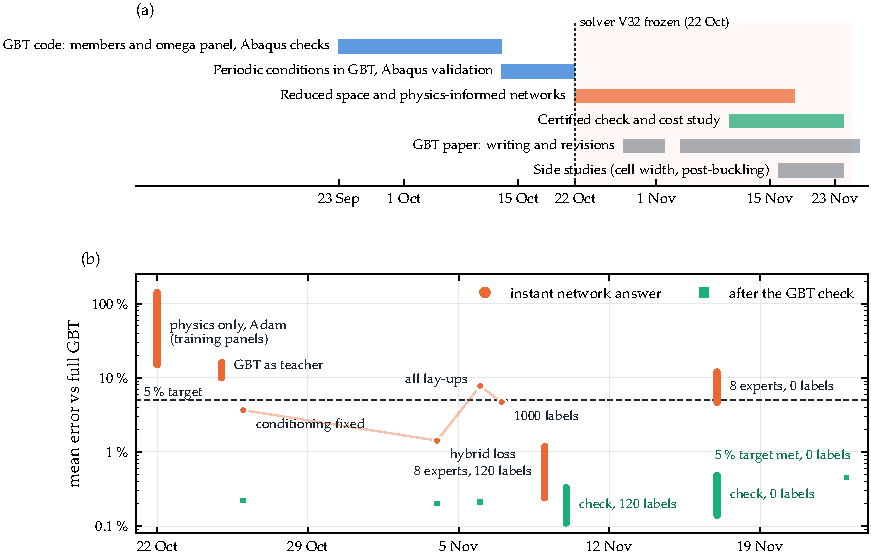
\includegraphics[width=\textwidth]{fig_history.pdf}
\caption{(a) Phases of the machine-learning work, 22 October to 23 November 2026 (in the gaps I worked on the GBT paper). (b) Mean error against full GBT of every network test, in the order in which it was run. All values are for unseen designs, except the first bar, which is the error on the 8--32 training panels themselves. Bars show the spread over designs or lay-ups.}
\label{fig:history}
\end{figure}

\subsection{One set of coordinates for every design (22 October)}
A network needs the same coordinates for every design, but GBT builds new cross-section modes on a new mesh for each one. My first idea, the modes of one quasi-isotropic reference panel, failed: on other lay-ups the load came out 20--130\pc{} too high, because the order of the modes changes with the laminate. An energy-weighted POD of the three lowest GBT modes of 64 panels on a fixed node layout worked; its 241 modes reproduce full GBT within 0.01--0.02\pc, whereas a panel's own 80 lowest modes would give 1.6\pc.

Along the length the problem was harder. The load enters through the eccentric foot, so the pre-buckling forces near the ends reach five times their mid-length value; many modes are concentrated at the ends (78\pc{} of one mode sat in the two end fifths) and the lowest loads are very close (16.02, 16.08 and 16.74\,N/mm in one example). A single wave with an envelope gave 1--13\pc{} error and one shape per wavenumber 4--55\pc. A Fourier series was accurate (within 0.1\pc) with 16--24 terms; a dictionary of fixed wavelengths plus end splines gave 0.05--0.27\pc{} and was the one I kept.

\subsection{A first physics-only network that would not train (22 October)}
With these coordinates I trained the first network on the GBT energy alone, by minimising the Rayleigh quotient of its predicted modes. For one panel it worked within a minute (0.2\pc), but for 8--32 panels the error was still 15--140\pc{} after 2000 Adam steps. Neural eigen-iteration targets, a wavenumber preconditioner (about 150 iterations), teacher modes as a guide and L-BFGS on free variables (7.8\pc{} after 300 iterations) were all slow. Only an exact stiffness solve converged quickly, in five iterations, which costs as much as a GBT solution. My conclusion at the time was that label-free training of one network for the whole family would cost about one GBT solution per design.

\subsection{GBT as a teacher (25 October)}
I therefore tried the opposite: a supervised network that learns the three lowest GBT loads and their mode subspace, with closed-form plate and column loads as extra inputs, and an ensemble of five networks with split-conformal intervals as a replacement for the window of Paper~1. With 160 training designs it reached 10--16\pc{} on unseen designs, better than the closed-form estimate (20\pc{} mean, 91\pc{} maximum) but worse than a Gaussian process (9.3\pc). Adding the GBT energy on 200 unlabelled designs did not help (16.1\pc), the error fell only slowly with more data (15\pc{} with 40 designs, 10\pc{} with 160), and the intervals were honest but far too wide ($\pm$46--81\pc, coverage 84--88\pc). I dropped this direction.

\subsection{Fixing the conditioning (26 October)}
Going back to the physics-only network, I looked for the reason of the slow training and found it in the numbers, not in the physics: in mode coordinates the condition number of $\mathbf K$ was between $10^{9}$ and $10^{19}$. Three changes solved it. First, energy-whitened coordinates, in which the strain energy is close to the squared length of the vector; an eigen-iteration then needs 7--13 steps instead of about 150, and fitting one design improved from 4.6\pc{} to 0.40\pc. Second, a function decoder instead of a linear output layer, because the modes of an unseen design lie 15--24\pc{} (in energy) outside the span of the modes of 45 other designs, so no fixed output basis can generalise. Third, natural-gradient training: in every outer step one physics eigen-step for every design, then a fit of the network to it. Table~\ref{tab:gen} shows how the error on unseen designs fell with these changes, first for clamped panels with symmetry sides.

\begin{table}[h]
\centering\small
\caption{Physics-only network, clamped ends, symmetry sides, industrial lay-ups: error on unseen designs (26 October).}
\label{tab:gen}
\begin{tabular}{@{}lrr@{}}
\toprule
Network and training & Instant $\Ncr$ & Rayleigh quotient of modes \\
\midrule
19 training designs (training error 1\pc) & 10\pc & 42\pc \\
259 designs, linear output layer & 9.4\pc & 10.6\pc \\
259 designs, function decoder, Adam & 9.5\pc & 20.6\pc \\
259 designs, function decoder, natural gradient & \textbf{5.0\pc} & 12.3\pc \\
\midrule
\multicolumn{3}{@{}l}{Check started from the last network: 2.8 / 1.9 / 1.1 / 0.54\pc{} after 3 / 5 / 8 / 12 steps} \\
\bottomrule
\end{tabular}
\end{table}

For the periodic cell with simply supported ends, the case of the GBT paper, the same network trained on 320 designs reached 3.65\pc{} on 32 unseen designs (9.77\pc{} maximum), and a 12-step check from its modes 0.22\pc.

\subsection{Learning from the suspicious designs, as in Paper 1 (27 October)}
In Paper~1, Abaqus labels were added only for suspicious panels. I tried the same with GBT as the oracle: a data term on the 10\pc{} of the designs where the network's number and its Rayleigh quotient disagreed most. It corrected exactly those designs but did not transfer to unseen ones (3.65--8.3\pc). The error stayed at about 3.6\pc{} for the number and 10\pc{} for the modes even on the training designs, which told me that the limit was how well the network can represent the modes, not the amount of data or the optimiser.

\subsection{Testing the plan against Paper 1 (3 November)}
Before going further I tested the first goal directly: I ran the full GBT code at the 22 Abaqus points of Paper~1 (cross-ply, symmetry side, simply supported ends). GBT deviates from Abaqus by 0.54\pc{} on average and by less than 1\pc{} everywhere, also at the tight pitch where the RBS model failed (Table~\ref{tab:abq}), and it finds the Abaqus half-wave number at all 22 points (Paper~1: 20). From then on GBT was both the physics and the reference, and Abaqus was not used in Paper~2.

\begin{table}[h]
\centering\small
\caption{Error against Abaqus at the 22 independent test points of Paper~1 (its Table~2; means and maxima computed from that table), mean / maximum.}
\label{tab:abq}
\begin{tabular}{@{}lrr@{}}
\toprule
Points & Paper 1 PINN & GBT \\
\midrule
All 22 & 2.53 / 10.80\pc & \textbf{0.54 / 0.97\pc} \\
Tight pitch, $b_s=124.25$\,mm (4 points) & 8.08 / 10.80\pc & \textbf{0.89 / 0.97\pc} \\
Other 18 points & 1.29 / 3.54\pc & \textbf{0.46 / 0.95\pc} \\
\bottomrule
\end{tabular}
\end{table}

A closer look at the best physics-only network showed that its number was biased high: above GBT in 27 of 32 designs, $+3.13$\pc{} on average. The network learns the Rayleigh quotient of its own imperfect modes, which always lies above the true load. After removing this bias the scatter was still 2.8\pc{} on average, and the error hardly correlated with $b_s$, $\beta$, the load itself or the gap between the two lowest loads (at most 0.2, with $\beta$).

\subsection{Physics, data or both (3--4 November)}
The bias raised the question whether GBT labels should enter the loss. A label costs about 13\,s per design, five times the physics data of a design (about 2.5\,s), so labels are not free but cheap. I trained three networks with identical settings: physics only, labels only, and both. In a first run with a constant learning rate the numbers were 3.65, 2.78 and 3.94\pc; the labels removed the bias, the physics loss gave the best mode shapes, and labels alone overfitted the shapes (11.8\pc{} on training against 18.9\pc{} on unseen designs). An ensemble of the three numbers reached 1.61\pc, but its spread did not predict the error (correlation 0.02), as in Paper~1, so an ensemble could not be the check.

I then repeated the comparison with clean training: 32 validation designs held out, a decaying learning rate, weight averaging, weights chosen on validation and test designs not looked at (Table~\ref{tab:loss}). With labels the number became much better, but it started to overfit after 8--10 outer steps, while the mode shapes kept improving until the end. Taking the number from the early weights and the modes from the final weights of the same network halved the error of a three-step check of the hybrid network (1.81\pc{} to 0.94\pc). I kept the hybrid loss: it remains a PINN, its labels come from GBT, and its check was the best.

\begin{table}[h]
\centering\small
\caption{Physics, data or both: clean retraining, periodic cell, 32 unseen designs (4 November).}
\label{tab:loss}
\begin{tabular}{@{}lrrr@{}}
\toprule
 & Physics only & Data only & Hybrid \\
\midrule
Instant number, mean / max & 4.48 / 11.89\pc & 1.21 / 4.79\pc & 1.42 / 4.35\pc \\
Bias of the number & $+4.47$\pc & $+0.05$\pc & $+0.55$\pc \\
Rayleigh quotient of the predicted modes & \textbf{11.95\pc} & 22.8\pc & 20.1\pc \\
Check after 12 steps, mean / max & 0.22 / 1.07\pc & 0.14 / 0.82\pc & 0.20 / 0.98\pc \\
\bottomrule
\end{tabular}
\end{table}

\subsection{A wider design space and the limit of one network (4--7 November)}
The next step was the full design space of Paper~1 ($b_s$ down to 124.25\,mm, $\beta$ up to 3.5, symmetry and periodic sides) with general as well as industrial lay-ups as input (38 inputs). Extending the space first meant checking the coordinates. The cross-section basis stayed accurate (at most 0.14\pc), but a long clamped panel was 5.3\pc{} off; the cause was a dictionary that was too short (longest half-wave 350\,mm), and two longer half-waves brought it to 0.012\pc. A denser wave series (11 half-waves of 25--1006\,mm) improved the short panels from 0.3 to 0.1\pc. When I refined the end splines, some values fell slightly below the reference, which should not happen for a Rayleigh--Ritz value. A check on a twice finer integration grid showed that this was an integration artefact of splines finer than the grid, not a better mode, so I limited the spline spacing to 1.5 grid spans. A few designs remained hard: end-localised local buckling with short waves on tight-pitch general lay-ups, where the worst one improved from 1.53\pc{} to 0.62\pc{} with finer end splines. Over the 1064 labelled training designs the space error was 0.061\pc{} on average and at most 0.49\pc.

Because something could still be wrong, I trained a pilot network early, on the first 223 labelled designs. It reached 7.75\pc{} on 100 unseen designs while fitting its training designs within 1.2\pc: clear overfitting. With all 1000 labels the error fell to about 4.7\pc{} and then stalled, again far above the 1.3\pc{} on the training designs. To find out whether the network was the problem, I trained an MLP ensemble, a Gaussian process and gradient boosting on the same 1000 labels: they reached 5.0--6.7\pc{} on average and about 28\pc{} at most, no better than the network. On realistic, industrial lay-ups alone, however, the Gaussian process reached 0.77\pc{} (4.2\pc{} maximum), while on the random ply-by-ply lay-ups 35 of 55 test designs were above 5\pc. The difficulty therefore lay in the random lay-ups, which are hard for any model, and even on these the 12-step check reached 0.21\pc.

\subsection{Lay-up experts and an industrial network (7--9 November)}
I decided to give every lay-up and side condition its own small network with only $b_s$ and $\beta$ as inputs: four standard lay-ups (the cross-ply of Paper~1, quasi-isotropic, $0^\circ$-rich and $\pm45^\circ$) times two side conditions, eight experts in total, each with 152 training and 40 unseen test designs. In addition I trained one network for all industrial lay-ups (38 inputs, 518 labels). Its validation error was best after eight rounds (1.60\pc) and then grew to 2.45\pc{} while the training error kept falling, so I kept the round-eight weights; on 45 unseen designs it reached 1.35\pc{} instantly and 0.14\pc{} after 12 check steps. No unseen lay-up is claimed.

A Gaussian process on the same 120 labels and the same two inputs then gave an important answer: it predicted the number as well as or better than the network for six of the eight experts. The network's advantage could therefore not be the number when many labels are available; it had to come from the mode shapes and the check.

\subsection{What the network really adds (9--17 November)}
I compared the network's modes as starting vectors of the check with simple alternatives that need no network: random vectors, and the GBT modes of the nearest labelled design copied into the new design (Figure~\ref{fig:check}a). The network saves two to three iterations against a random start, but a copied neighbour does as well, and the nearest of 120 labelled designs is better. Interestingly, the network's modes have a better Rayleigh quotient than the copied ones (24\pc{} against 63\pc{} for the nearest of ten designs), yet the check converges more slowly from them: the network learns smooth shapes with a low energy quotient, not the detail the iteration needs. Mixing network and neighbour modes made the check worse, a correction network on top of the copied modes did not beat the plain copy, and neighbour modes stretched to the new length were numerically unstable in one to three designs.

On 16 November I tried to improve the mode shapes directly and stopped after two hours, for two reasons. The exact first mode is on average 98.2\pc{} a single harmonic of the panel length, but the remaining 2\pc{} carry the stiff membrane and end-zone part of the energy: cutting the exact modes to their strongest harmonics made the Rayleigh quotient wrong by a factor of more than 60. And one iteration costs only about 0.17\,s, while the fixed cost of a check is about 5\,s, so even a perfect start could save at most about 1.5\,s. A final look at the modes as information confirmed the picture: the network's modes are closer in shape to GBT than copied ones (MAC 0.39--0.40 against 0.29), but they find the right number of half-waves in only 39--44\pc{} of the designs, because the lowest modes are often only 2--5\pc{} apart; after 12 check steps the half-wave number is right in 318 of 320 designs.

\section{Results}

\subsection{The eight experts}
Figure~\ref{fig:experts}a shows the mean errors of the eight experts on 40 unseen designs each. Without labels, trained on the GBT energy alone, the instant answer is 4.7--11.9\pc{} off and too high in 319 of 320 designs; with 120 labels it is 0.24--1.18\pc{} off (maximum 0.87--4.92\pc). After 12 check steps the error is 0.11--0.48\pc{}, practically the same with and without labels, because the check uses the mode shapes, which come from the physics. The label study in Figure~\ref{fig:experts}b shows that labels are what makes the instant number usable, and that with few labels a Gaussian process predicts the number better than the network.

\begin{figure}[t]
\centering
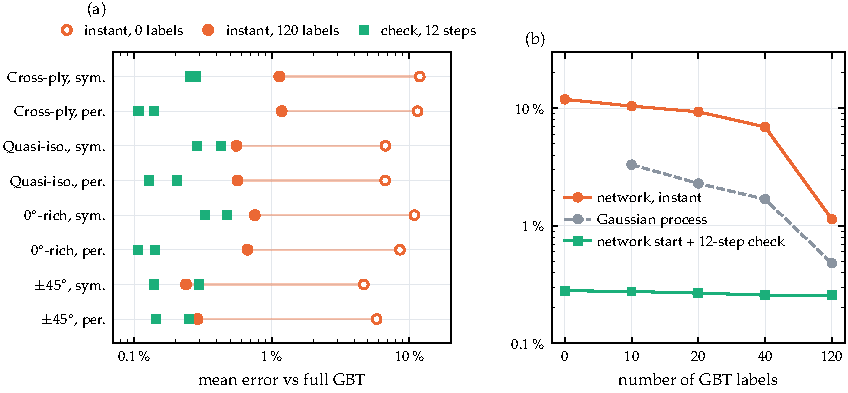
\includegraphics[width=\textwidth]{fig_experts.pdf}
\caption{(a) Mean error of the eight experts on 40 unseen designs each (sym.: symmetry side, per.: periodic cell). (b) Label study for the cross-ply expert, symmetry side.}
\label{fig:experts}
\end{figure}

\subsection{The certified check and its error estimate}
With the network's role clear, the effort went into the check. Profiling showed where its time goes: most of it is the pre-buckling state of the new design (2.4--9.7\,s), not the iteration. Solving the pre-buckling state in the shared basis was slower, not faster. A four times coarser pre-buckling mesh cut the check to 36--53\pc{} of a full GBT solution, but for industrial lay-ups the load dropped by up to 0.11\pc{} below full GBT, so it was no longer an upper bound; I went back to the exact pre-buckling state, which costs 63\pc{} (5 steps) to 76\pc{} (12 steps) of a full solution and was never below it. Cheaper parts (coarser meshes, single precision) saved at most about 0.3\,s, and a Kato--Temple lower bound was still 14\pc{} wide after five steps while costing more than the check itself.

For the error estimate I compared three candidates built from the residual. The squared residual was close to the true error but not safe (too small in 10\pc{} of the cases after five steps); the squared residual divided by the gap to the next eigenvalue was safe but 5--90 times too large. The plain relative residual $\eta$ worked (Figure~\ref{fig:check}b): over 760 checks and five iteration counts it was never below the true error (3800 of 3800 cases), it is conservative by a factor of 3--11 in the median, and its rank correlation with the true error reaches 0.88, equally with and without labels. The standard deviation of a Gaussian process, in comparison, correlated with its own error only weakly (0.06--0.47), and for the cross-ply expert its $\pm2\sigma$ band covered only 60--62\pc{} of the designs with 10--20 labels. The limit of $\eta$ is that it measures the iteration error inside the reduced space, not the fixed error of that space against full GBT (at most 0.49\pc, 0.06\pc{} on average, over 1064 designs).

\begin{figure}[t]
\centering
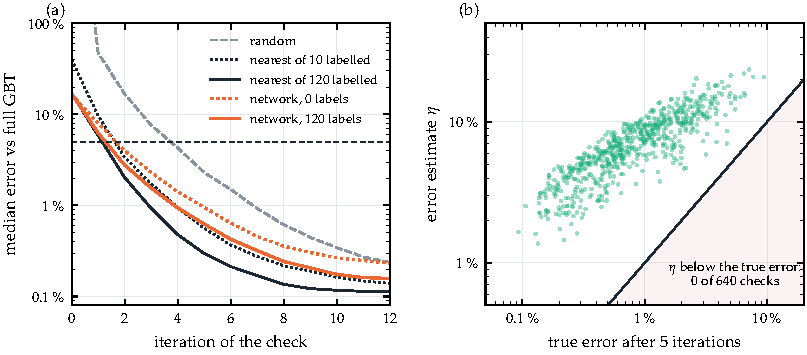
\includegraphics[width=\textwidth]{fig_check.pdf}
\caption{(a) Median error against the iteration of the check for different starting vectors, 320 unseen designs. (b) Error estimate against the true error after five iterations, 640 checks; the shaded region, where the estimate would be too small, is empty.}
\label{fig:check}
\end{figure}

\subsection{Cost of a 5\,\% target}
Following the count of Abaqus calls in Paper~1, I asked what it costs to give every one of the 320 unseen designs an answer within 5\pc{} of full GBT (Table~\ref{tab:cost}). The check stops when $\eta\le5\pc$; a design that never gets there would receive a full GBT solution, which was never needed. The check meets the target on every design without any labels, already from a random start, in 7.3--7.9\,s per design instead of 10.7\,s. A Gaussian process needed 80 labels per lay-up (40 were not enough) and gives neither a guarantee nor the mode shapes. The network start saves about two iterations, or about 0.5\,s per design, so its training of about two hours per expert pays off only after about 2400 designs; most of the time of a check (about 4.5\,s) goes into building the matrices of the design.

\begin{table}[h]
\centering\small
\caption{Cost of a 5\pc{} target on 320 unseen designs (totals over the eight experts; offline time includes labels, operators and, for the network, training).}
\label{tab:cost}
\begin{tabular}{@{}lrrrrc@{}}
\toprule
Method & GBT solves & Offline & Per design & Error, mean / max & Upper bound \\
\midrule
Full GBT for every design & 320 & -- & 10.7\,s & 0 / 0\pc & exact \\
GP, 40 labels per lay-up & 320 & 1.0\,h & $<1$\,ms & 0.75 / 7.68\pc & no \\
GP, 80 labels per lay-up & 640 & 1.9\,h & $<1$\,ms & 0.57 / 4.76\pc & no \\
GP, 120 labels per lay-up & 960 & 2.9\,h & $<1$\,ms & 0.40 / 3.65\pc & no \\
Check, random start & 0 & -- & 7.9\,s & 0.38 / 1.18\pc & yes \\
Check, nearest of 10 labelled & 80 & 0.2\,h & 7.3\,s & 0.32 / 1.20\pc & yes \\
Check, nearest of 120 labelled & 960 & 2.9\,h & 7.4\,s & 0.30 / 1.66\pc & yes \\
Check, network, 0 labels & 0 & 18.5\,h & 7.4\,s & 0.45 / 2.51\pc & yes \\
Check, network, 120 labels & 960 & 19.1\,h & 7.3\,s & 0.36 / 1.83\pc & yes \\
\bottomrule
\end{tabular}
\end{table}

\section{Scope and limitations}
The periodic condition keeps the cell width constant, as in the validated GBT code and the Abaqus models of both papers; without this constraint $\Ncr$ would be higher by 2.8--4.0\pc{} for the cross-ply cell and by 21--160\pc{} for the other lay-ups ($\beta=1.5$), so the results are conservative, and this will be stated clearly. The check takes 63--76\pc{} of a full GBT solution, mostly for building the matrices; the error estimate covers only the iteration error; the study is restricted to simply supported ends, $\beta\ge0.75$, four lay-ups and the industrial set, with no unseen lay-up.

\section{Conclusions and next steps}
\begin{enumerate}[leftmargin=*]
\item GBT as the physics removes the RBS error of Paper~1 (0.54\pc{} against 2.53\pc{} at its Abaqus points) and makes Abaqus unnecessary.
\item A shared reduced space gives every design the same coordinates, with a critical load at most 0.49\pc{} (0.06\pc{} on average) from full GBT over 1064 designs; this is what makes a network over many designs possible.
\item A PINN trains on the GBT energy only once the conditioning is fixed. Without labels it learns the mode shapes but not an unbiased number; 120 GBT labels make the instant number accurate to 0.24--1.18\pc. One network for arbitrary lay-ups stalls near 5\pc, as do plain data models; lay-up experts solve this.
\item The certified check replaces the $-15\pc/{+3}\pc$ window: it is an upper bound in the reduced space, independent of the order of the designs, and its label-free error estimate was never below the true error. It meets a 5\pc{} target on all 320 unseen designs without labels.
\item Compared honestly with simple alternatives, the network's start saves only a few iterations, and with few labels a Gaussian process predicts the number better. The main contribution is therefore the GBT engine with the certified check; the network adds the instant answer and the mode shapes.
\end{enumerate}
The next steps are to choose the journal and write the paper from this report. Two ideas are left open: repeating the label study for a second lay-up, and, since the pre-buckling state is the expensive part of the check, learning its end-zone part with a network instead of solving it.

\begin{thebibliography}{9}\small
\bibitem{p1} A.\,M. Elsayed, N. Kharghani, S. El Yaakoubi-Mesbah, C. Mittelstedt, A hybrid physics-informed neural network framework for local buckling prediction of stiffened composite panels with epistemic uncertainty quantification, \emph{Composite Structures} 399 (2026) 120959.
\bibitem{gbt} A.\,M. Elsayed, N. Kharghani, C. Mittelstedt, Periodic boundary conditions in generalized beam theory for the buckling analysis of omega-stringer-stiffened composite panels, manuscript under review (2026).
\bibitem{sc} N. Silvestre, D. Camotim, First-order generalised beam theory for arbitrary orthotropic materials, \emph{Thin-Walled Structures} 40 (2002) 755--789.
\bibitem{lobpcg} A.\,V. Knyazev, Toward the optimal preconditioned eigensolver: locally optimal block preconditioned conjugate gradient method, \emph{SIAM Journal on Scientific Computing} 23 (2001) 517--541.
\end{thebibliography}

\end{document}
